\section{Robustness}

\begin{figure}%
	\centering
	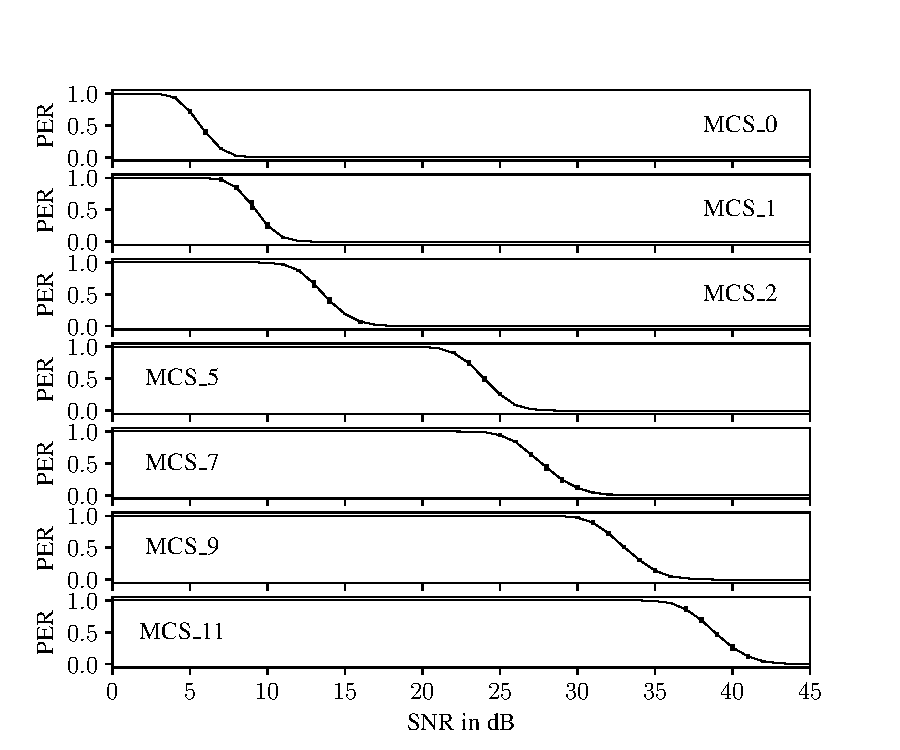
\includegraphics[width=0.95\textwidth]{figures/MCS_PER_to_SNR.pdf}
	\caption{Achieved Goodput and theoretical Datarate of two WiFi 6 stations in Ad-Hoc Mode with a \ac{GI} of \SI{3200}{\nano\second} and a bandwidth of \SI{40}{\mega\hertz} in regards to the number of the chosen \ac{MCS} and \ac{CR} and whether \ac{DCM} is enabled}%
	\label{fig:PER_SNR_MCS}%
\end{figure}

\begin{figure}%
	\centering
	
\includegraphics[width=0.95\textwidth]{figures/GI_PER_to_SNR.pdf}
	\caption{Achieved Goodput and theoretical Datarate of two WiFi 6 stations in Ad-Hoc Mode with a \ac{GI} of \SI{3200}{\nano\second} and a bandwidth of \SI{40}{\mega\hertz} in regards to the number of the chosen \ac{MCS} and \ac{CR} and whether \ac{DCM} is enabled}%
	\label{fig:PER_SNR_GI}%
\end{figure}

\begin{figure}%
	\centering
	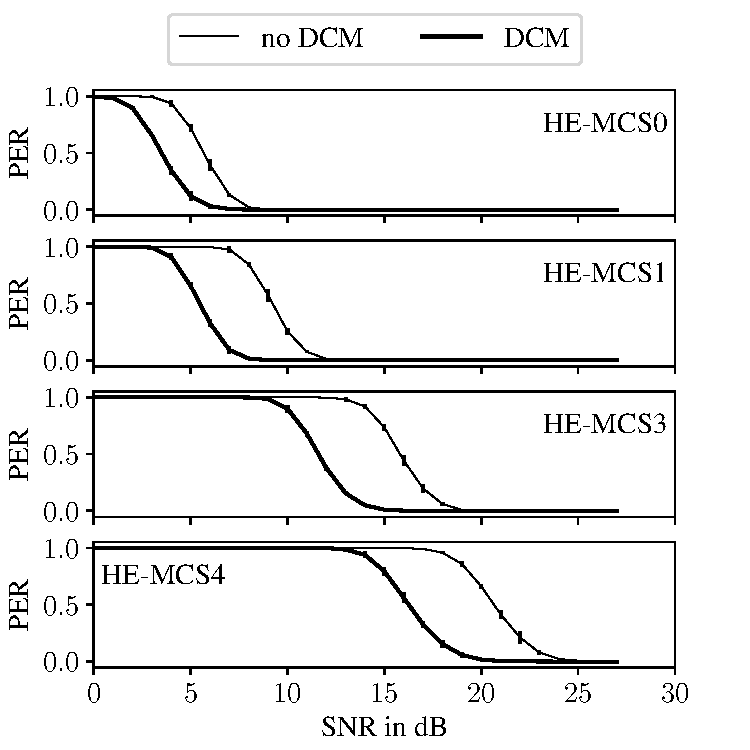
\includegraphics[width=0.95\textwidth]{figures/DCM_PER_to_SNR.pdf}
	\caption{Achieved Goodput and theoretical Datarate of two WiFi 6 stations in Ad-Hoc Mode with a \ac{GI} of \SI{3200}{\nano\second} and a bandwidth of \SI{40}{\mega\hertz} in regards to the number of the chosen \ac{MCS} and \ac{CR} and whether \ac{DCM} is enabled}%
	\label{fig:PER_SNR_DCM}%
\end{figure}

\begin{figure}%
	\centering
	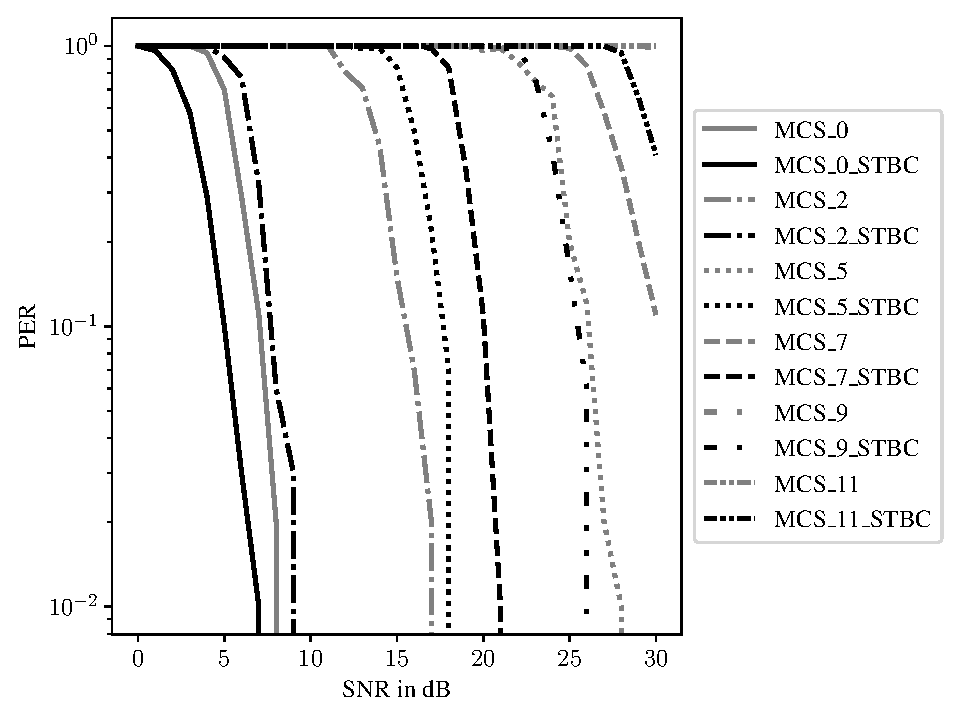
\includegraphics[width=0.95\textwidth]{figures/STBC_PER_to_SNR.pdf}
	\caption{Achieved Goodput and theoretical Datarate of two WiFi 6 stations in Ad-Hoc Mode with a \ac{GI} of \SI{3200}{\nano\second} and a bandwidth of \SI{40}{\mega\hertz} in regards to the number of the chosen \ac{MCS} and \ac{CR} and whether \ac{DCM} is enabled}%
	\label{fig:PER_SNR_STBC}%
\end{figure}